% This is part of Un soupçon de mathématique sans être agressif pour autant
% Copyright (c) 2014
%   Laurent Claessens
% See the file fdl-1.3.txt for copying conditions.

\begin{exercice}\label{exosmath-0824}

    Un charpentier doit couper des poutres de bonne longueur pour créer un triangle isocèle. La poutre transversale horizontale fait \unit{8}{\meter} et l'inclinaison du toit est de \unit{40}{\degree}. 
    \begin{enumerate}
        \item
            Dessiner un schéma à l'échelle. Préciser l'échelle choisie (par exemple \unit{1}{\centi\meter} sur la feuille représente \unit{1}{\meter} dans la réalité).
        \item
            En déduire la longueur des poutres inclinées.
    \end{enumerate}

    Vous pouvez vous inspirer du dessin suivant\cite{EKNooAsTWza} (qui n'est pas à l'échelle)
    \begin{center}
    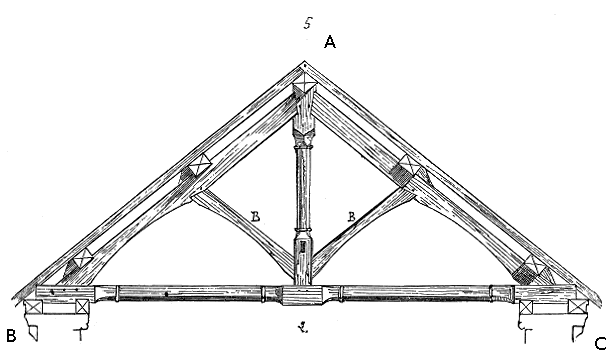
\includegraphics[width=0.7\linewidth]{Charpenteetjambettes2.png}
    \end{center}
    Sur ce dessin nous aurions la longueur \( BC=\SI{8}{\meter}\) et les angles \( \widehat{ABC}=\widehat{ACB}=\SI{40}{\degree}\). Les poutres inclinées dont nous voulons savoir la longueur sont \( [AB]\) et \( [AC]\).
    
\corrref{smath-0824}
\end{exercice}
